

\begin{frame}{Волновая функция}{}
    \textbf{Wikipedia $^*$ :}\\
    Волновая функция — комплекснозначная функция, используемая для описания чистого квантового состояния системы. Обычно
    функция имеет комплексные значения, а для одной частицы это функция пространства и времени. Изменение волновой
    функции сравнимо с поведением волны.
    \vspace{0.5cm} \\

    \textbf{Физический смысл волновой функции} заключается в том, что согласно копенгагенской интерпретации квантовой механики
    плотность вероятности нахождения частицы в данной точке пространства в данный момент времени считается равной
    квадрату абсолютного значения волновой функции этого состояния в координатном представлении.
\end{frame}


\begin{frame}{Уравнение Шредингера}
    Итак обзовем оператором Н (Гамильтониан):
      $$ H =  \frac{-\hbar^2}{2m} \nabla^2 + V   $$
      тогда :
      \Huge  
      $$ H\Psi=E\Psi $$
      \small 
      Для решения этого уравнения надо найти значения Е и волновой функции. Это уравнение относится к типу дифференциальных
      уравнений с собственными значениями, где оператор действующий на функцию возвращает произведение скалярной
      величины на функцию.
  \end{frame}

\begin{frame}{Операторы}
    \textbf{Ожидаемое значение} (можно рассматривать как среднее значение) какого либо свойства: энергии, положения, линейного  момента, можно определить
      с помощью оператора.\\
      \textbf{Пример:} гамильтониан это оператор для энергии
      можно сказать, что зная волновую функцию:
      $$ E= \frac{\int \dot{\Psi} H \Psi \partial r}{\int \dot{\Psi}\Psi \partial r} $$
      Интегрировать надо по всем осям от $-\infty$ до $+\infty$.  \\
      Надо учитывать, что волновая может быть сложным числом и поэтому комплексная составляющая указывается явно.
\end{frame}

\begin{frame}{Одно-электронный атом}
%       \footnotesize{
    $ H =  \frac{-\hbar^2}{2m} \nabla^2 - \frac{Ze^2}{4\pi\epsilon _0 r}   $  или  в упрощенных единицах: 
    $ H =  \frac{1}{2} \nabla^2 - \frac{Z}{r}  $\\
Так как система имеет сферическую симметрию, то можно представить волновую функцию в сферических координатах.

\[ \left(- \frac{\hbar^2}{2} \nabla^2  - \frac{Ze^2}{4 \pi \epsilon_0 r} \right) \psi(r,\theta, \psi) = E \psi(r, \theta, \psi) \] 
расскроем оператор Лапласа:
\small
\[ \frac{\hbar^2}{2} \left[ \frac{1}{r^2} \frac{\partial }{\partial r} \left( r^2 \frac{
            \partial \psi}{\partial r}\right) + \frac{1}{r^2 \sin \theta} \frac{\partial }{\partial \theta} \left( \sin \theta \frac{\partial
            \psi}{\partial \theta}\right) + \frac{1}{r^2 \sin^2 \theta} \frac{\partial^2 \psi}{\partial \phi^2} \right] - \frac{Ze^2}{ 4 \pi
    \epsilon_0 r} \psi= E \psi \]
\end{frame}
\begin{frame}{Одно-электронный атом}
    разделив переменные : $ \Psi(r,\theta,\phi) =R(r)Y(\theta,phi)$
\[ \left[ \frac{\hbar^2}{2} \frac{1}{r^2} \frac{\partial }{\partial r} \left( r^2 \frac{
            \partial \psi}{\partial r}\right)  - \frac{Ze^2}{ 4 \pi
    \epsilon_0 r}\right] R(r) = \lambda R(r) \] 

\[ \frac{\hbar^2}{2} \left[   \frac{1}{r^2 \sin \theta} \frac{\partial }{\partial \theta} \left( \sin \theta \frac{\partial
            \psi}{\partial \theta}\right) + \frac{1}{r^2 \sin^2 \theta} \frac{\partial^2 \psi}{\partial \phi^2} \right]Y(\theta,\phi)= -\lambda
Y(\theta,\phi )\]
Накладывая стандартные условия (периодичность и нормировку), переходим к следующему слайду
\end{frame}
\begin{frame}{Одно-электронный атом водорода}
    Итак решения :
    \begin{itemize}
        \item Радиальная функция \[ R_{n,l}(r)=R_{\infty}(r)b_0\exp{\left(\frac{\mu Ze^2r}{2\pi\epsilon_0\hbar^2n}\right)}\qquad \]
        \item Зенитиная часть \[
                P_l^m=(1-x^2)^{\frac{m}{2}}\left(a_0\sum_{n=0}^{\infty}\frac{a_{2n}}{a_0}x^{2n}+a_1\sum_{n=1}^{\infty}\frac{a_{2n+1}}{a_1}x^{2n+1}\right)
            \] где \[a_{n+2}=\frac{(n+m)(n+m+1)-A}{(n+1)(n+2)}a_n\qquad.\]
        \item Азимутальная часть \[      \Phi_m(\phi)=c_1{\rm e}^{{\rm i}m\phi} \]
    \end{itemize}      

\end{frame}

\begin{frame}{Одно-электронный атом водорода}
    \footnotesize{

\[\psi_{n\ell m}(r,\vartheta,\varphi) = \sqrt {{\left (  \frac{2}{n a_0} \right )}^3\frac{(n-\ell-1)!}{2n(n+\ell)!} } e^{-
\rho / 2} \rho^{\ell} L_{n-\ell-1}^{2\ell+1}(\rho) Y_{\ell}^{m}(\vartheta, \varphi ); \quad \]
$  L_{n-\ell-1}^{2\ell+1}(\rho)$ - Обобщённый полином Лагерра степени n-l-1 ; 
\( \rho=\frac{2r}{na_0}\)\\
$Y_{\ell}^{m}(\vartheta, \varphi ) $ - Сферическая гармоника  ;
\\
}
\vspace{0.2cm}
\small{
Где n,l,m это основные квантовые числа
\begin{itemize}
    \item n- основное число (1,2,3..)
    \item l – орбитальное число (0,1,2.. n-1)
    \item m – магнитное число (-l..+l)
\end{itemize}
}
\end{frame}

\begin{frame}{Одно-электронный атом, волновые функции}
    \centering
    \begin{tabular}{ccc|c}
        n & l & m & функция \rule[-0.9ex]{0pt}{0pt}\\
        \hline 
        1 & 0 & 0 & ${1\over \sqrt{\pi}}\left({1\over a_0}\right)^{3/2}e^{-r/a_0}$  \\[0.5cm]
        2 & 0 & 0 & ${1\over 4\sqrt{2\pi}}\left({1\over a_0}\right)^{3/2}\left(2-{r\over a_0}\right)e^{-r/2a_0}$ \\[0.5cm]
        2 & 1 & 0 & $ {1\over 4\sqrt{2\pi}}\left({1\over a_0}\right)^{3/2} {r\over a_0}e^{-r/2a_0}\cos{\theta}$ \\[0.5cm]
        2 & 1 & -1;1 & ${1\over 8} \sqrt{1\over \pi} \left({1\over a_0}\right)^{3/2}{r\over a_0}e^{-r/2a_0}\sin{\theta}e^{\pm
            i\phi}$ \\[0.5cm]
    \end{tabular}
\end{frame}


\begin{frame}{Метод самосогласованного поля, SCF}
    Межэлектронное отталкивание вычисляется как влияние общего (среднего) поля на данный электрон, и это зависит только
    от положения данного электрона. 
    \\
    Это приближение позволяет повторить разделение переменных  в сферических  координатах.
    \[ H^{ссп}_i= \frac{-\hbar^2}{2m} \nabla^2 - \frac{Ze^2}{4\pi\epsilon_0r_i} + \sum_{j\neq i}^{N}\left\langle \left (
        \frac{e^2}{4\pi\epsilon_0r_{ij}} \right ) \right\rangle _j
        \]
        Эти уравнения называют одноэлектронными. \\
        Суть решения состоит в итеративном изменении параметров в функциях, до тех пор пока изменение энергии не станет
        незначительным.

\end{frame}


\begin{frame}{Перейдём к молекулам:}
        Решать напрямую уравнения ХФ по отношению к молекулам, тяжело. Одной из успешных стратегий является
        введение базисных функций, т.е. волновая функция это комбинация одноэлектронных базисных функций и некоторых
        коэффициентов. \\
        \[ \psi_i =\sum _{\nu=1}^{K}c_{\nu i}\psi_\nu ; \quad \frac{\partial E}{\partial c_{\nu i}} =0 
         \]
     \end{frame}


\section{Базисы}


\begin{frame}{Базис}
    \begin{itemize}
        \item \textbf{Базисный набор это:} набор математических функций используемых для описания электронных орбиталей атомов в молекуле. 
        \item \textbf{Ограниченный базис:} базисные функции в которых \textbf{не происходит} изменение параметров в функции в ходе расчёта  молекулярных орбиталей.
        \item  \textbf{Неограниченный базис:} базисные функции в которых  \textbf{происходит} изменение параметров в функции в ходе расчёта
    молекулярных орбиталей.
    \end{itemize}
    Часто такими математическими функциями является гауссиан:
    \[ \psi = d e^{-\alpha r^2} \]
\end{frame}

\begin{frame}{Пример STO-2G для Н:}
    \begin{columns}
        \begin{column}{0.5\textwidth}
    \small\begin{tikzpicture} %[xscale=.5,yscale=.5]
  \begin{axis}[
    height=5.5cm,width=6cm,
    xmin=-0,xmax=8,
    ymin=0,ymax=0.6, 
    xlabel=$r$,
    ylabel=$\Psi$
  ]
    \addplot[white!40!blue] gnuplot[id=psi]{sqrt(1/pi)*exp(-x)};
    \addplot[white!40!red] gnuplot[id=g1]{0.67*(2*0.15/pi)**0.75*exp(-0.15*x*x)};
    \addplot[white!40!green] gnuplot[id=g2]{0.43*(2*0.85/pi)**0.75*exp(-0.85*x*x)};
    \addplot[white!40!cyan] gnuplot[id=g2g1]{%
    0.43*(2*0.85/pi)**0.75*exp(-0.85*x*x)+
    0.67*(2*0.15/pi)**0.75*exp(-0.15*x*x)
    };
    %\legend{$\chi$,$c_1g_1$,$c_2g_2$,$c_1g_1+c_2g_2$}
  \end{axis}
\end{tikzpicture}
\end{column}
        \begin{column}{0.5\textwidth}
        \[ \psi = \sum _1 ^2 c e^{-\alpha r^2}\] 
        \[ \psi = c_1g_1 + c_2g_2 \]
\begin{tabular}{c c c} 
    \hline 
    & $\alpha$ & $c$ \\
    \hline
  1 & 0.151623 & 0.678914 \\
  2 & 0.851819 & 0.430129 \\
    \hline
\end{tabular}
\end{column}
\end{columns}
\small$\epsilon$ = -0.4665819 a.u. = 12.697 eV. \\В реальности 13.606 eV. И ошибка 87.7 кДж/моль
\end{frame}

\begin{frame}{Гауссианы:}
\[
    1s=Ne^{\alpha r^2} ;   \quad 
    2p_x=Ne^{\alpha r^2}x; \quad
    2p_y=Ne^{\alpha r^2}y; \quad
    2p_z=Ne^{\alpha r^2}z; \quad
\]
\[
    3d_{xx}=Ne^{\alpha r^2}x^2;  \quad
    3d_{xy}=Ne^{\alpha r^2}xy;   \quad
    3d_{xz}=Ne^{\alpha r^2}xz;   \quad
\]                             
\[    
    3d_{yy}=Ne^{\alpha r^2}y^2;  \quad
    3d_{yz}=Ne^{\alpha r^2}yz ;  \quad
    3d_{zz}=Ne^{\alpha r^2}z^2;  \quad
\]
\[
4f_{xxx}=Ne^{\alpha r^2}x^3   ; \quad
4f_{xxy}=Ne^{\alpha r^2}x^{2}y; \quad
4f_{xxz}=Ne^{\alpha r^2}x^{2}z; \quad
\]
И так далее.
\end{frame}

\begin{frame}{Описания базисных наборов для программы GAUSSIAN:}
    Общий вид обозначений от Поупл и коллег:  \textbf{M-ijk..G}
    \begin{itemize}
        \item \textbf{М} – количество ограниченных  гаусианов на один не валентный электрон
        \item Наличие двух  и более букв после “-” означает, что  валентные электроны описываются 2 и более функциями,
            каждая из     которых состоит из линейной комбинации \textbf{i,j,k}  гауссианов
        \item * -Означает, что для тяжёлый атомов используются не только гауссианы характерные для конкретной орбитали,
            но и     гауссианы следующей орбитали. \\
         \vspace{0.5cm}
         Например для углерода в \textbf{3-21*G}:  у валентных электронов с 3 гауссианами прибавляется  6 гауссианов для d-орбиталей. 
        \end{itemize}
\end{frame}

\begin{frame}{Описания базисных наборов для программы GAUSSIAN:}
    \begin{itemize}
\item ** то же самое, что и * ,но добавляются 3 гауссиана для р-орбиталей к гауссианам Н и Не.
    \vspace{1cm}

\item  + Означает добавление дополнительных гауссианов тех же орбиталей, но с маленьким значением α. Этот шаг нужен для
    точного счёта систем где значительная электронная плотность удалена от ядра: электронные пары, анионы.
\end{itemize}
\end{frame}




\begin{frame}{Уравнение Шредингера}
	\[ \left ( -\frac{\hbar^2}{m}( \left [ \frac{\partial^2}{\partial x} + \frac{\partial^2}{\partial y} + \frac{\partial^2}{\partial z} \right ] +V \right )
		\Psi (r,t) = i\hbar \frac{\partial \Psi(r,t)}{\partial t} 
	\]
	Или:
	\[
		H\Psi = E\Psi ; \quad H= \frac{-\hbar^2}{m} \nabla^2 - \frac{Ze^2}{4\pi \varepsilon_0 r}
	\]
	Современные базисы предполагают примерно 60 функций на атом. Итого: 900 функций на аминокислоту.
    \vspace{1cm}
    \begin{itemize}
    \item  Можно апроксимировать электронную плотность уравнениями класической физики.
   \end{itemize}

\end{frame}


\begin{frame}{Молекулярная механика (MM)}{}
 \begin{itemize}
  \item
  В ММ электронная структура атома замещается на достаточно простые уравнения с параметрами.
\vspace{0.2cm}
  \item
   Наборы параметров называются силовыми полями.
\vspace{0.2cm}
  \item
      Используется допущение Борна-Оппенгеймера (электроны быстро адаптируются к движению ядер)
\vspace{0.2cm}
  \item
	 Расчёт энергии происходит на основе положения ядер.
\vspace{0.2cm}
  \item
	  Упрощения позволяют работать с большими системами
\vspace{0.2cm}
  \item
	   В некоторых случаях ММ подходы могут давать результаты, сравнимые по точности с методами QM.
\vspace{0.2cm}
 \end{itemize}
\end{frame}


\begin{frame}{Простое уравнение силового поля (СП)}

\begin{center}
\[ U=\sum_{bonds}{ \frac{k_i}{2} ( l_i - l_0)^2} + \sum_{angles}{ \frac{k_i}{2} ( \phi_i - \phi_0)^2} + \sum_{torsions}
{ \frac{V_n}{2} (1 + cos(n\omega - \gamma))} + \]
    \[ + \sum_{i=1}^N \sum_{j=i+1}^N  \left (   4 \epsilon_{ij} \left [ \left ( \frac{\sigma_{ij}}{r_{ij}} \right )^{12} - \left ( \frac{\sigma_{ij}}{r_{ij}} \right )^6  \right ] + 
\frac{q_i q_j}{ 4\pi \epsilon_0 r_{ij}} \right ) 
\]
\vspace{0.5cm}

    \begin{tikzpicture} [xscale=.7,yscale=.6]
%bond
        \node[circle,draw,minimum size=0cm,fill=purple!80] (b1) at (0,10) {};
        \node[circle,draw,minimum size=0cm,fill=purple!80] (b2) at (2,10) {};
        \node[circle,draw,minimum size=0cm,fill=purple!80] (a1) at (4,10) {};
        \node[circle,draw,minimum size=0cm,fill=purple!80] (a2) at (6,10) {};
        \node[circle,draw,minimum size=0cm,fill=purple!80] (a3) at (5,9 ) {};
        \node[circle,draw,minimum size=0cm,fill=purple!80] (d1) at (7,9) {};
        \node[circle,draw,minimum size=0cm,fill=purple!80] (d2) at (7.5,10) {};
        \node[circle,draw,minimum size=0cm,fill=purple!80] (d3) at (9.5,10) {};
        \node[circle,draw,minimum size=0cm,fill=purple!80] (d4) at (10,11) {};
%        \draw[fill=blue!20] (5,10) circle [radius=.1];
        \draw [ color   = white,   thick,  <-> ] (b1) -- (b2) node[midway,below] {\scriptsize Связи};
        \draw [ color   = white,   thick,   ] (a1) -- (a3);
        \draw [ color   = white,   thick,   ] (a2) -- (a3);
        \draw[<->, >=latex', shorten >=2pt, shorten <=2pt, bend right=-45, thick, dashed] 
            (a1) to node[above] {\scriptsize Углы} (a2); 
        \draw [ color   = white,   thick,   ] (d1) -- (d2);
        \draw [ color   = white,   thick,   ] (d2) -- (d3);
        \draw [ color   = white,   thick,   ] (d3) -- (d4);
        \draw[->,dashed,>=latex',thick ] (8.5,10) .. controls +(-90:15mm) and +(120:15mm) ..
        (8.5,10);
        \node at (8,11) {\scriptsize Торсионные углы} ;
% non-bond
        \node[circle,draw,minimum size=0cm,fill=red!50] (q1) at (0,7) {+};
        \node[circle,draw,minimum size=0cm,fill=blue!50] (q2) at (1,8) {-};
        \node[circle,draw,minimum size=0cm,fill=blue!50] (q3) at (2,7.5) {-};
      \node at (1,6){\scriptsize Кулоновские взаимодействия};


        \node[circle,draw,minimum size=0cm,fill=green!50] (v1) at (8,7) {};
        \node[circle,draw,minimum size=0cm,fill=green!50] (v2) at (6,7) {};
        \node[circle,draw,minimum size=0cm,fill=green!50] (v3) at (7,6) {};

      \node at (7,8.3){\scriptsize Ван-дер-Ваальсовы взаимодействия};
        \node[circle,draw,minimum size=1cm,dashed] (w1) at (8,7) {};
        \node[circle,draw,minimum size=1cm,dashed] (w2) at (6,7) {};
        \node[circle,draw,minimum size=1cm,dashed] (w3) at (7,6) {};

    \end{tikzpicture}
\end{center}


\end{frame}




\section{Силовые поля}
\begin{frame}{Основные особенности силовых полей}{}
\begin{itemize}
\vspace{0.2cm}
  \item
Большинство параметров неотделимо от поля.
\vspace{0.2cm}
  \item
Параметризация ММ сильно зависит от целей исследования.
\vspace{0.2cm}
  \item
Большинство  силовых  полей параметризованы для воспроизведения структуры.
\vspace{0.2cm}
  \item
Силовые поля — это результат оптимизации параметров.
\vspace{0.2cm}
  \item
Силовые поля — это эмпирически найденные данные.
\end{itemize}
\end{frame}


\begin{frame}{Типы атомов в СП}{}
\includegraphics[width=0.7\textwidth]{his.png}
\end{frame}

\section{Ковалентные взаимодействия}

\begin{frame}{Потенциал для описания связи}{}
\begin{minipage}{10cm}
\begin{columns}
\begin{column}{0.5\textwidth}
Потенциал Морзе 
$$ U(l)=D_e \{  1-e^{[-a(l-l_0)]} \}^2 $$
Более распространённый
$$ U(l)=\frac{{k_i}}{2} ( l_i - l_0)^2 $$
\end{column}
\begin{column}{0.5\textwidth}
 \small\begin{tikzpicture} %[xscale=.5,yscale=.5]
  \begin{axis}[
    height=5.5cm,width=7cm,
    %xmin=1.5,xmax=2.4,%ymin=0,ymax=4, 
    xlabel=$r$,
    ylabel=$E$
  ]
  \addplot+[raw gnuplot, draw=white!40!blue, mark=none, smooth] gnuplot[id=m]{%
  set xrange [1.95:2.4]; plot (1-exp(-20*(x-2)))**2 };
  %\legend{$\left(1-e^{-20(x-2)}\right)^2$}
  \end{axis}
\end{tikzpicture}
\end{column}
\end{columns}
\end{minipage}
\end{frame}

\begin{frame}{Параметры при описании связи}
   \begin{center}

%\rowcolors{1}{White}{Gray}
%\rowcolors{2}{gray!10}{}\tiny
%\rowcolors[]{1}{blue!20}{blue!10}
%
       \[ E=\frac{k}{2}(r-r_0)^2\]

%\rowcolors[]{1}{blue!20}{blue!10}
\begin{tabular}{c c c}
\textbf{связь} & \textbf{r\textsubscript{0},A} & \textbf{k, kcal mol\textsuperscript{-1}A\textsuperscript{-2}} \\[0.2cm]
    \hline
C\textsubscript{sp3}-C\textsubscript{sp3} & 1.523 & 317 \\[0.2cm]
    \hline
C\textsubscript{sp2}-C\textsubscript{sp2} & 1.337 & 690 \\[0.2cm]
    \hline
C\textsubscript{sp2}-O\textsubscript{sp2} & 1.208 & 777 \\[0.2cm]
    \hline
C\textsubscript{sp3}-N\textsubscript{sp3} & 1.438 & 367 \\[0.2cm]
    \hline

\end{tabular}
\end{center}
\end{frame}

\begin{frame}{Кубический и прочие варианты}
\begin{center}
 \small\begin{tikzpicture} %[xscale=.5,yscale=.5]
  \begin{axis}[
    height=5.5cm,width=7cm,
    %xmin=1.5,xmax=2.4,
    ymin=0,ymax=0.04, 
    xlabel=$r$,
    ylabel=$E$,
    legend style={cells={anchor=west},legend pos=outer north east, draw=none}
  ]
  \addplot+[raw gnuplot, draw=white!40!blue, mark=none, smooth] gnuplot[id=m]{%
  set xrange [1.95:2.4]; plot 0.01*(1-exp(-20*(x-2)))**2 };
  \addplot+[raw gnuplot, draw=white!40!red , mark=none, smooth] gnuplot[id=p1]{%
  set xrange [1.9:2.4]; 
  plot 2*(x-2)**2 };
  \addplot+[raw gnuplot, draw=white!40!green, mark=none, smooth] gnuplot[id=p2]{%
  set xrange [1.9:2.4]; 
  plot 2*(x-2)**2*(1-4*(x-2)-8*(x-2)**2) };
  %\legend{\tiny$\left (1-e^{-20(x-2)}\right)^2$,\tiny$2(x-2)^2$,\tiny$2(x-2)^2(1-4(x-2)-8(x-2)^2)$}
  \end{axis}
  \end{tikzpicture}
\end{center}
\[ U = \frac{k_i}{2} ( l_i - l_0)^2 ( 1-k'( l_i - l_0)- k''( l_i - l_0)^2 - k'''( l_i - l_0)^3 - k''''( l_i - l_0)^4
\dots ) \]
\end{frame}

\begin{frame}{Потенциал валентного угла}
    \[ U(\phi)=\frac{k_i}{2} ( \phi_i - \phi_0)^2 \]
или
\[ 
    \begin{array}{c}
    U(\phi)=\frac{k_i}{2} ( \phi_i - \phi_0)^2 ( 1-k'( \phi_i - \phi_0) - k''( \phi_i - \phi_0)^2 - \\
    \\
    - k'''( \phi_i -\phi_0)^3 - k''''( \phi_i - \phi_0)^4 \dots ) 
\end{array}
\]
\end{frame}

\begin{frame}{Потенциал торсионного угла}
	\[ U(\omega) = \sum_{torsions} \frac{V_n}{2} (1 + cos(n\omega - \gamma)) \quad \]%
    Рассмотрим О-С-С-О (сахар в ДНК) \hspace{1cm}
%\setcrambond{2pt}{}{}%
\tiny%\setatomsep{3em}
\chemfig[atom sep=2em,cram width=2pt]{HO-[2,0.5,2]?<[7,0.7](-[2,0.5]OH)-[,,,,line width=2pt]
	(-[6,0.5]OH)>[1,0.7](-[6,0.5]OH)-[3,0.7]
O-[4]?(-[2,0.3]-[3,0.5]OH)}\newline
\begin{center}
\begin{tikzpicture} %[xscale=.5,yscale=.5]
  \begin{axis}[
    height=5cm,width=5cm,
    %xmin=1.5,xmax=2.4,
    ymin=0,ymax=1.4, 
    xlabel=$\omega$,
    ylabel=$E$,
   % legend style={cells={anchor=west},legend pos=outer north east, draw=none}
  ]
  \addplot+[raw gnuplot, draw=white!40!blue, mark=none, smooth] gnuplot[id=m]{
  set xrange [-180:180]; 
  plot 0.25*(1+cos(3*pi*x/180)) };
  \addplot+[raw gnuplot, draw=white!40!red , mark=none, smooth] gnuplot[id=p1]{
  set xrange [-180:180]; 
  plot 0.25*(1+cos(2*pi*x/180)) };
  %\legend{$\frac{1}{4}(1+cos(3\pi\omega))$,$\frac{1}{4}(1+cos(2\pi\omega))$}
  \end{axis}
  \end{tikzpicture}
\begin{tikzpicture} %[xscale=.5,yscale=.5]
  \begin{axis}[
    height=5cm,width=7cm,
    %xmin=1.5,xmax=2.4,
    ymin=0,ymax=1.4, 
    xlabel=$\omega$,
  %  ylabel=$\omega$,
   % legend style={cells={anchor=west},legend pos=outer north east, draw=none}
  ]
  \addplot+[raw gnuplot, draw=white!40!blue, mark=none, smooth] gnuplot[id=m]{%
  set xrange [-180:180]; 
  plot 0.25*(1+cos(3*pi*x/180))+ 0.25*(1+cos(2*pi*x/180)) };
  %\legend{$\frac{1}{4}(1+cos(3\pi\omega))+\frac{1}{4}(1+cos(2\pi\omega))$}
  \end{axis}
  \end{tikzpicture}
\end{center}
\end{frame}

\begin{frame}{Потенциал торсионного угла}
    \[ U(\omega)= \frac{V_1}{2} (1 + cos\omega )+ \frac{V_2}{2} (1 + cos2\omega )+ 
        \frac{V_3}{2} (1 + cos3\omega)\dots\]
 \begin{itemize}
\vspace{0.2cm}
  \item
Для поля ММ2 используют три члена.
\vspace{0.2cm}
  \item
Поле OPLS использует ряды с 4-ю слагаемыми.
  \end{itemize}

\vspace{0.2cm}
\small\[ U(\omega)= \frac{1}{2} \left [ F_1(1 + cos\omega )+F_2 (1 - cos2\omega )+ F_3  (1 + cos3\omega )+ F_4  (1 -
cos4\omega ) \right ] \]
\end{frame}


\begin{frame}{"Неправильные" торсионные углы}
\begin{columns}
\begin{column}{0.5\textwidth}
\includegraphics[width=1.\textwidth]{impr.png}
\end{column}
\begin{column}{0.5\textwidth} 
    \[ U(\omega)= {V_1} (1 - cos\omega ) \]
    \[ U(\omega)= {V_1} (\omega - \omega_0)^2 \]
\end{column}
\end{columns}
Для циклобутанона кислород должен находиться в одной плоскости с1,с2,с3. \\
Используют  потенциал, где перечисление не 1-2-3-4, а 1-4-2-3 
\end{frame}


\begin{frame}{Кросс-составляющие в силовых полях}
Кросс-составляющие отражают зависимость состояния одной связи или угла от состояния соседней связи. \\
Существуют: strech-strech, strech-bend, strech-torsion
\vspace{0.5cm}
\begin{columns}
\begin{column}{0.3\textwidth}
    \begin{tikzpicture} [xscale=.7,yscale=.6]
%bond
        \node[circle,draw,minimum size=0cm,fill=purple!80] (a1) at (4,10) {};
        \node[circle,draw,minimum size=0cm,fill=purple!80] (a2) at (6,10) {};
        \node[circle,draw,minimum size=0cm,fill=purple!80] (a3) at (5,9 ) {};
        \node[] (a4) at (3,11 ) {};
        \node[] (a5) at (7,11 ) {};
%        \draw[fill=blue!20] (5,10) circle [radius=.1];
        \draw [ color   = white,   thick,   ] (a1) -- (a3);
        \draw [ color   = white,   thick,   ] (a2) -- (a3);
        \draw [ color   = white,   thick, ->,dashed ] (a1) -- (a4);
        \draw [ color   = white,   thick, ->,dashed ] (a2) -- (a5);
        \draw[<->, >=latex', shorten >=2pt, shorten <=2pt, bend right=-45, thick, dashed] 
            (a1) to node[above] {} (a2); 
    \end{tikzpicture}
\end{column}
\begin{column}{0.7\textwidth} 
    \[ U(l_1 ,l_2)= \frac{K_{l_1 l_2}}{2} (l1 - l_{1,0})^2 (l2 - l_{2,0})^2 \]
    \[U(l_1 ,l_2,\phi)= \frac{K_{l_1 l_2 \phi }}{2} [(l1 - l_{1,0})^2 +(l2 - l_{2,0})^2](\phi -\phi_0) \]
\end{column}
\end{columns}
\end{frame}

\section{Нековалентные взаимодействия}
\begin{frame}{Нековалентные взаимодействия}
 \begin{itemize}
  \item
Нековалентные взаимодействия являются определяющими в формировании структуры биополимеров. 
\vspace{0.2cm}
  \item
Так как эти взаимодействия реализуются через пространство, то часто они описываются как функции, обратно пропорциональные расстоянию между двумя атомами.
  \end{itemize}
\end{frame}

\begin{frame}{Электростатические  взаимодействия}
Допустим, что поверхность единичного потенциала можно представить зарядами в центрах атомов.\\
Тогда электростатические взаимодействия будут описываться по закону Кулона:
\[ U(q_1 ,q_2)= \frac{q_1 q_2}{4\pi \epsilon_0 \epsilon_r r_{ij}} ;  \]
\[ U= \sum_{i=1}^{N_A} \sum_{j=1}^{N_B} \frac{q_i q_j}{4\pi \epsilon_0 \epsilon_r r_{ij}}  \]
\end{frame}

\begin{frame}{Электростатические  взаимодействия}
Очевидно, что количество вычислений растет значительно быстрее количества частичных зарядов. \\
Существуют следующие упрощения:\vspace{0.5cm}
 \begin{itemize}
\item
Разрастание центрального мультиполя (ММ малых молекул)
\vspace{0.2cm}
  \item
Двойное обрезание
\vspace{0.2cm}
  \item
Потенциал реакционного поля
\vspace{0.2cm}
  \item
Суммирование Эвальда
  \end{itemize}
\end{frame}

\begin{frame}{Двойное обрезание}

    \centering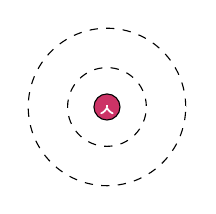
\begin{tikzpicture} [xscale=.7,yscale=.6]
%bond
        \node[circle,draw,minimum size=0cm,fill=purple!80] (a1) at (0,0) {};
        \node[circle,draw,minimum size=1cm,dashed] (a2) at (0,0) {};
        \node[circle,draw,minimum size=2cm,dashed] (a3) at (0,0 ) {};
        \draw [ color   = white,   thick, -> ] (a1) -- (a2);
        \draw [ color   = white,   thick, -> ] (a1) -- (a3.east);
    \end{tikzpicture}
    \\
    
	%\centering \includegraphics[width=0.25\textwidth]{twin_co.png} \\
Для сферы А мы считаем все частичные заряды, а для сферы А-В мы будем считать взаимодействие групп зарядов с нашим атомом.
		
\[ U_1= \sum_{i=1}^{N_A}  \frac{q_1 q_i}{4 \pi \epsilon_0 \epsilon_r r_{1} } + 
\sum_{j=1}^{N_{group}}  \frac{q_1 q_j}{4 \pi \epsilon_0 \epsilon_r r_{1j} }  \]
%\sum_{j=1}^N_{group}  \frac{q_1 q_{j} }{4\pi \epsilon_0 \epsilon_r r_{1j}} \]

\end{frame}

\begin{frame}{Потенциал реакционного поля}
Основная идея: мы считаем, что за некоторым расстоянием плотность заряда одинаковая, и, следовательно, известна некая
диэлектрическая проницаемость среды.\\
\vspace{0.5cm}

\[ U_{ij}=   \frac{q_1 q_i}{4\pi \epsilon_0 \epsilon_r r_{1i}}  \left [ 1 + \frac{ \epsilon_{rf} - \epsilon_r}{ 2\epsilon_{rf} + 
\epsilon_r}\frac{r_{ij}^3}{ r_c^3} \right ] - \frac{q_1 q_i}{4\pi \epsilon_0 \epsilon_r r_c}\frac{3\epsilon_{rf}}{ 2
\epsilon_rf + \epsilon_r}  \]
\end{frame}


\begin{frame}{Суммирование Эвальда}{}
Основная идея: нам нужно учитывать не только заряды в ближайшем окружении, но и, как в кристалле, заряды, находящиеся в соседних ячейках.\\
\[ U_{ij}=  \sum_{x=1}^{N_x} \sum_{y=1}^{N_y} \sum_{z=1}^{N_z} \sum_{i=1}^{N} \sum_{j=1}{N}{\frac{q_i q_i}{4\pi \epsilon_0 \epsilon_r r_{ij}}} \]
Это сходится, но очень медленно.
\end{frame}

\begin{frame}{Суммирование Эвальда}{}
%\small
Эвальд предложил перевести этот ряд в сумму 2-ух быстро сходящихся рядов и константы.
\[
    \begin{array}{l}
	U=U_{dir} + U_{rec} +U_0   \\
    \\
 U_{dir}=f/2 \sum_{i,j}^{N} \sum_{x=1}^{N_x}  \sum_{y=1}^{N_y}  \sum_{z=1}^{N_z} {q_i q_i \frac{erfc(\beta_{r_{ij},n})}{r_{ij,n}}}  \\
 \\
 U_{rec}= \frac{f}{2}\pi V \sum_{i,j}^{N}  q_i q_i \sum_{m_x} \sum_{m_y} \sum_{n_z} {\frac{exp(-\pi m/\beta )^2 +2 \pi i m (r_i \cdot r_j)}m^2} \\
 \\
U_0=\frac{f \beta}{\sqrt{\pi}} \sum_{i}^{N} q_{i}^2 
\end{array}
\]
Где бета - это параметр, определяющий соотношение прямого и обратного взаимодействий
\end{frame}


\begin{frame}{Суммирование Эвальда vs двойное обрезание}
\includegraphics[width=0.45\textwidth]{b1.png}
\includegraphics[width=0.45\textwidth]{b2.png}
\begin{columns}
\begin{column}{0.5\textwidth}
Self-assembly with PME
\end{column}
\begin{column}{0.5\textwidth} 
Self-assembly  with Cut-off
\end{column}
\end{columns}
\end{frame}

\begin{frame}{Ван-дер-Ваальсовы взаимодействия}
 \begin{itemize}
  \item
В основе природы Ван-дер-Ваальсовых взаимодействий лежат электронные эффекты: дисперсионные и обменные. 
\vspace{0.2cm}
  \item
В принципе, рассчитать такие эффекты можно в QM, но это далеко не тривиальная задача. 
\vspace{0.2cm}
  \item
В ММ нам надо считать такие взаимодействия быстро, на сегодняшний день наиболее часто используют потенциал Леонарда-Джонса:
\vspace{0.2cm}
  \end{itemize}

  \[ 
      U_{VdW}= \sum_{i=1}^N \sum_{j=i+1}^N  4\epsilon_{ij}  
      \left [ 
      \left ( \frac{\sigma_{ij}}{r_{ij}} \right )^{12} -
      \left ( \frac{\sigma_{ij}}{r_{ij}} \right )^6 
      \right ] 
  \]

\end{frame}


\begin{frame}{Ван-дер-Ваальсовы взаимодействия}
Наряду с потенциалом Леонарда-Джонса используют потенциал Букингама:

\[ V_{bh}(r_{ij})= A_{ij}exp(-B_{ij}r_{ij})-\frac{C_{ij}}{r^6_{ij}} \]
%\[ U_{VdW}= \epsilon \left [ 6 \frac {\alpha -6} exp [ -\alpha(r/r_m-1)] -\frac{\alpha}{\alpha-6} \left (\frac{r}{r_m} \right )^6  \right ] \]
\end{frame}

\begin{frame}{Взаимодействия между разными типами атомов}
Константы для разных типов атомов будут разные. Для их определения существуют правила смешивания:\\
\[\sigma_{AB}= \frac{1}{2}\left( \sigma_{AA} + \sigma_{BB}\right ) \]
\[\epsilon_{AB}= \sqrt{ \epsilon_{AA} \epsilon_{BB}} \]
Это не единственный вариант правила смешивания, но такой подход наиболее распространён для моделирования биологических систем 
\end{frame}


\begin{frame}{Различия для 1-4 взаимодействий}{}
 \begin{itemize}
  \item
Так как 1-4 взаимодействия могу быть уже учтены в описании торсионного угла, то может быть, что силовых полях такие нековалентные взаимодействия не учитываются.
\vspace{0.2cm}
  \item
В полях семейства AMBER, 1-4 VdW взаимодействия всё-таки учитываются, но их потенциал делится на 2.
  \end{itemize}
\end{frame}


\begin{frame}{Водородные связи}{}
 \begin{itemize}
  \item
В силовых  полях водородная связь часто описывается как комбинация Ван-дер-Ваальсовых и Кулоновских взаимодействий
\vspace{0.2cm}
  \item
Существуют силовые поля, где водородная связь задаётся своим потенциалом на основе потенциала Леонарда-Джонса 10-12:
  \end{itemize}
  \[ U_{HB}=\frac{A}{r}^{10} -\frac{C}{r}^{12} \]
\end{frame}

\begin{frame}{Водородные связи}{}
Для точного описания водородной связи вносят поправки, учитывающие геометрию водородной связи:\\
\vspace{0.2cm}

\begin{columns}
\begin{column}{0.5\textwidth}
	\[ U_{HB}=\left ( \frac {C}{d^6} - \frac {D}{d^4 } \right ) \cos^m \theta \] 
\end{column}
\begin{column}{0.5\textwidth}
    \tiny\chemfig{-[7](-[1])=[6]\lewis{7:,Y}@{p1}-[@{a1}6,,,,dash pattern=on 2pt off 2pt]H-[@{a2}5]X-[6](-[5])-[7]}
    \chemmove{%
        \draw[white!40!blue,](a1).. controls +(180:3mm) and +(135:3mm).. node[left]{$\theta$} (a2);
        \draw[white!40!red,](p1).. controls +(-45:2mm) and +(0:2mm).. node[right]{$\omega$} (a1);
    }



%	\includegraphics[width=0.4\textwidth]{hb.png}	
\end{column}
\end{columns}
\vspace{0.2cm}

\[ U_{HB}=\left ( \frac {A}{r^{10}_{H\dots Ac}} - \frac {C}{r^{12}_{H\dots Ac} } \right ) \cos^2 \theta_{\color{white!40!blue}Don-H\dots Acc}
    cos^4 \omega_{\color{white!40!red}{LP-Acc \dots H}}
\] 
\end{frame}

\section{Варианты ММ}
\begin{frame}{Эффективный парный потенциал}
		Для системы из 1000 частиц существует 499500 парных  взаимодействий и 166167000 тройных взаимодействий.\\
		\vspace{1cm}
		\textbf{Выход есть:}
			\begin{itemize}
				\item Использование парного потенциала с 'правильной' параметризацией. 
				\item Пример: использовать большие частичные заряды для фазы, чем для одной молекулы.
				\item Это работает для воды. 1.85 D vs 2.6 D
			\end{itemize}
\end{frame}




\begin{frame}{Модели воды}
	\begin{itemize}
		\item	Вода - достаточно сложный объект.
		\item	Важно, что модель воспроизводила как свойства одной молекулы, так и свойства фазы.
	\end{itemize}
    \vspace{.5cm}

    \textbf{Существуют три основных  класса моделей:}

	\begin{itemize}
		\item Простые модели
		\item Поляризуемые модели
		\item Ab initio модели 
	\end{itemize}
\end{frame}

\begin{frame}{Модели воды}
	\textbf{Простые модели} \\
	\vspace{.5cm}
    \centering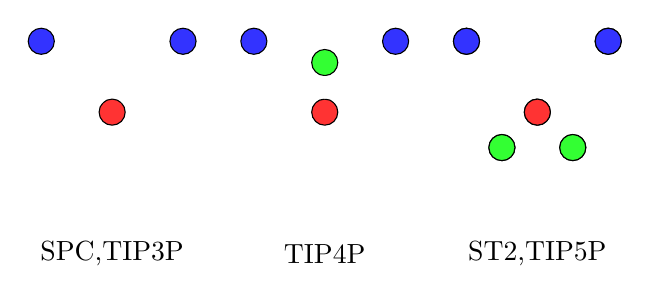
\begin{tikzpicture} [xscale=.9,yscale=.9]
        \node[circle,draw,minimum size=0cm,fill=blue!80] (a1) at (1,10) {};
        \node[circle,draw,minimum size=0cm,fill=blue!80] (a2) at (3,10) {};
        \node[circle,draw,minimum size=0cm,fill=red!80] (a3) at (2,9 ) {};
%        \draw[fill=blue!20] (5,10) circle [radius=.1];
        \draw [ color   = white,   thick,   ] (a1) -- (a3);
        \draw [ color   = white,   thick,   ] (a2) -- (a3);
      \node at (2, 7) {SPC,TIP3P}; 
        \node[circle,draw,minimum size=0cm,fill=blue!80] (b1) at (4,10) {};
        \node[circle,draw,minimum size=0cm,fill=blue!80] (b2) at (6,10) {};
        \node[circle,draw,minimum size=0cm,fill=red!80] (b3) at (5,9 ) {};
        \node[circle,draw,minimum size=0cm,fill=green!80] (b4) at (5,9.7 ) {};
%        \draw[fill=blue!20] (5,10) circle [radius=.1];
        \draw [ color   = white,   thick,   ] (b1) -- (b3);
        \draw [ color   = white,   thick,   ] (b2) -- (b3);
        \draw [ color   = white,   thick,   ] (b4) -- (b3);
      \node at (5, 7) {TIP4P}; 
        \node[circle,draw,minimum size=0cm,fill=blue!80] (d1) at (7,10) {};
        \node[circle,draw,minimum size=0cm,fill=blue!80] (d2) at (9,10) {};
        \node[circle,draw,minimum size=0cm,fill=red!80]  (d3) at (8,9 ) {};
        \node[circle,draw,minimum size=0cm,fill=green!80](d4) at (7.5,8.5 ) {};
        \node[circle,draw,minimum size=0cm,fill=green!80](d5) at (8.5,8.5 ) {};
%        \draw[fill=blue!20] (5,10) circle [radius=.1];
        \draw [ color   = white,   thick,   ] (d1) -- (d3);
        \draw [ color   = white,   thick,   ] (d2) -- (d3);
        \draw [ color   = white,   thick,   ] (d4) -- (d3);
        \draw [ color   = white,   thick,   ] (d5) -- (d3);
      \node at (8, 7) {ST2,TIP5P};

        \node[circle,draw,minimum size=0cm,fill=blue!80] (d1) at (7,10) {};
        \node[circle,draw,minimum size=0cm,fill=blue!80] (d2) at (9,10) {};
        \node[circle,draw,minimum size=0cm,fill=red!80]  (d3) at (8,9 ) {};
        \node[circle,draw,minimum size=0cm,fill=green!80](d4) at (7.5,8.5 ) {};
        \node[circle,draw,minimum size=0cm,fill=green!80](d5) at (8.5,8.5 ) {};


% non-bond
    \end{tikzpicture}\\
	\vspace{.5cm}
В большинстве случаев применяют так называемые rigid body варианты моделей, хотя и существуют модели, где связи представлены потенциалами.
\end{frame}

\begin{frame}{Модели воды}
	\textbf{Поляризуемые модели}\\
	\vspace{.5cm}
	Есть два подхода:
    \begin{itemize}
		\item Смещать центр заряда кислорода относительно центра атома
		\item Добавить точки вокруг кислорода, в которых может меняться заряд
		\end{itemize}
    \centering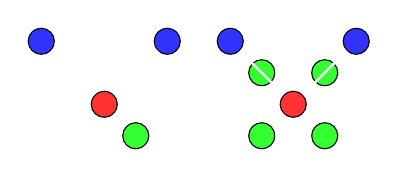
\begin{tikzpicture} [xscale=.8,yscale=.8]
%bond
        \node[circle,draw,minimum size=0cm,fill=blue!80] (b1) at (4,10) {};
        \node[circle,draw,minimum size=0cm,fill=blue!80] (b2) at (6,10) {};
        \node[circle,draw,minimum size=0cm,fill=red!80] (b3) at (5,9 ) {};
        \node[circle,draw,minimum size=0cm,fill=green!80] (b4) at (5.5,8.5 ) {};
%        \draw[fill=blue!20] (5,10) circle [radius=.1];
        \draw [ color   = white!40!white,   thick,   ] (b1) -- (b3);
        \draw [ color   = white!40!white,   thick,   ] (b2) -- (b3);
        \draw [ color   = white!40!white,   thick,   ] (b4) -- (b3);


        \node[circle,draw,minimum size=0cm,fill=blue!80] (d1) at (7,10) {};
        \node[circle,draw,minimum size=0cm,fill=blue!80] (d2) at (9,10) {};
        \node[circle,draw,minimum size=0cm,fill=red!80]  (d3) at (8,9 ) {};
        \node[circle,draw,minimum size=0cm,fill=green!80](d4) at (7.5,8.5 ) {};
        \node[circle,draw,minimum size=0cm,fill=green!80](d5) at (8.5,8.5 ) {};
        \node[circle,draw,minimum size=0cm,fill=green!80](d6) at (7.5,9.5 ) {};
        \node[circle,draw,minimum size=0cm,fill=green!80](d7) at (8.5,9.5 ) {};
%        \draw[fill=blue!20] (5,10) circle [radius=.1];
        \draw [ color   = white!40!white,   thick,   ] (d1) -- (d3);
        \draw [ color   = white!40!white,   thick,   ] (d2) -- (d3);

        \draw [ color  = white!40!white,   dashed ] (d4) -- (d5);
        \draw [ color  = white!40!white,   dashed ] (d5) -- (d7);
        \draw [ color  = white!40!white,   dashed ] (d4) -- (d6);
        \draw [ color  = white!40!white,   dashed ] (d6) -- (d7);
        \draw [ color  = white!40!white,   dashed ] (d3) -- (d5);
        \draw [ color  = white!40!white,   dashed ] (d3) -- (d4);
% non-bond
    \end{tikzpicture}\\
	\end{frame}

\begin{frame}{Силовые поля с объединёнными атомами }
	Основная идея: не учитывать атомы водорода, не принимающие участие в образовании водородной связи. К массе атома без водорода добавляется 1.\\
   \vspace{0.5cm}
	Есть проблема:\\
   \vspace{0.5cm}
    \centering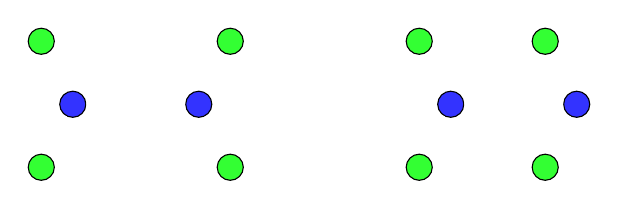
\begin{tikzpicture} [xscale=.8,yscale=.8]
%bond
        \node[circle,draw,minimum size=0cm,fill=blue!80] (b1) at (4,10) {};
        \node[circle,draw,minimum size=0cm,fill=blue!80] (b2) at (6,10) {};
        \node[circle,draw,minimum size=0cm,fill=green!80] (b3) at (3.5,11 ) {};
        \node[circle,draw,minimum size=0cm,fill=green!80] (b4) at (3.5,9 ) {};
        \node[circle,draw,minimum size=0cm,fill=green!80] (b5) at (6.5,11 ) {};
        \node[circle,draw,minimum size=0cm,fill=green!80] (b6) at (6.5,9 ) {};
        \draw [ color   = white!40!white,   thick,   ] (b1) -- (b2);
        \draw [ color   = white!40!white,   dashed,   ] (b1) -- (b3);
        \draw [ color   = white!40!white,   dashed,   ] (b1) -- (b4);
        \draw [ color   = white!40!white,   dashed,   ] (b2) -- (b6);
        \draw [ color   = white!40!white,   dashed,   ] (b2) -- (b5);

        \draw [ color   = white!40!white,   thick, <->  ] (7,10) -- (9,10);

        \node[circle,draw,minimum size=0cm,fill=blue!80] (d1) at (10,10) {};
        \node[circle,draw,minimum size=0cm,fill=blue!80] (d2) at (12,10) {};
        \node[circle,draw,minimum size=0cm,fill=green!80] (d3) at (9.5,11 ) {};
        \node[circle,draw,minimum size=0cm,fill=green!80] (d4) at (9.5,9 ) {};
        \node[circle,draw,minimum size=0cm,fill=green!80] (d5) at (11.5,11 ) {};
        \node[circle,draw,minimum size=0cm,fill=green!80] (d6) at (11.5,9 ) {};
        \draw [ color   = white!40!white,   thick,   ] (d1) -- (d2);
        \draw [ color   = white!40!white,   dashed,   ] (d1) -- (d3);
        \draw [ color   = white!40!white,   dashed,   ] (d1) -- (d4);
        \draw [ color   = white!40!white,   dashed,   ] (d2) -- (d6);
        \draw [ color   = white!40!white,   dashed,   ] (d2) -- (d5);

% non-bond
    \end{tikzpicture}\\
%	\hspace{2cm}\includegraphics[width=0.7\textwidth]{uf.eps} 
\end{frame}

\begin{frame}{Силовое поле Martini с объединёнными атомами }
        Основная идея: объединять четыре тяжелых атома и связанные ими атомы
    водорода в одну частицу. 
    \\
    \begin{center}
      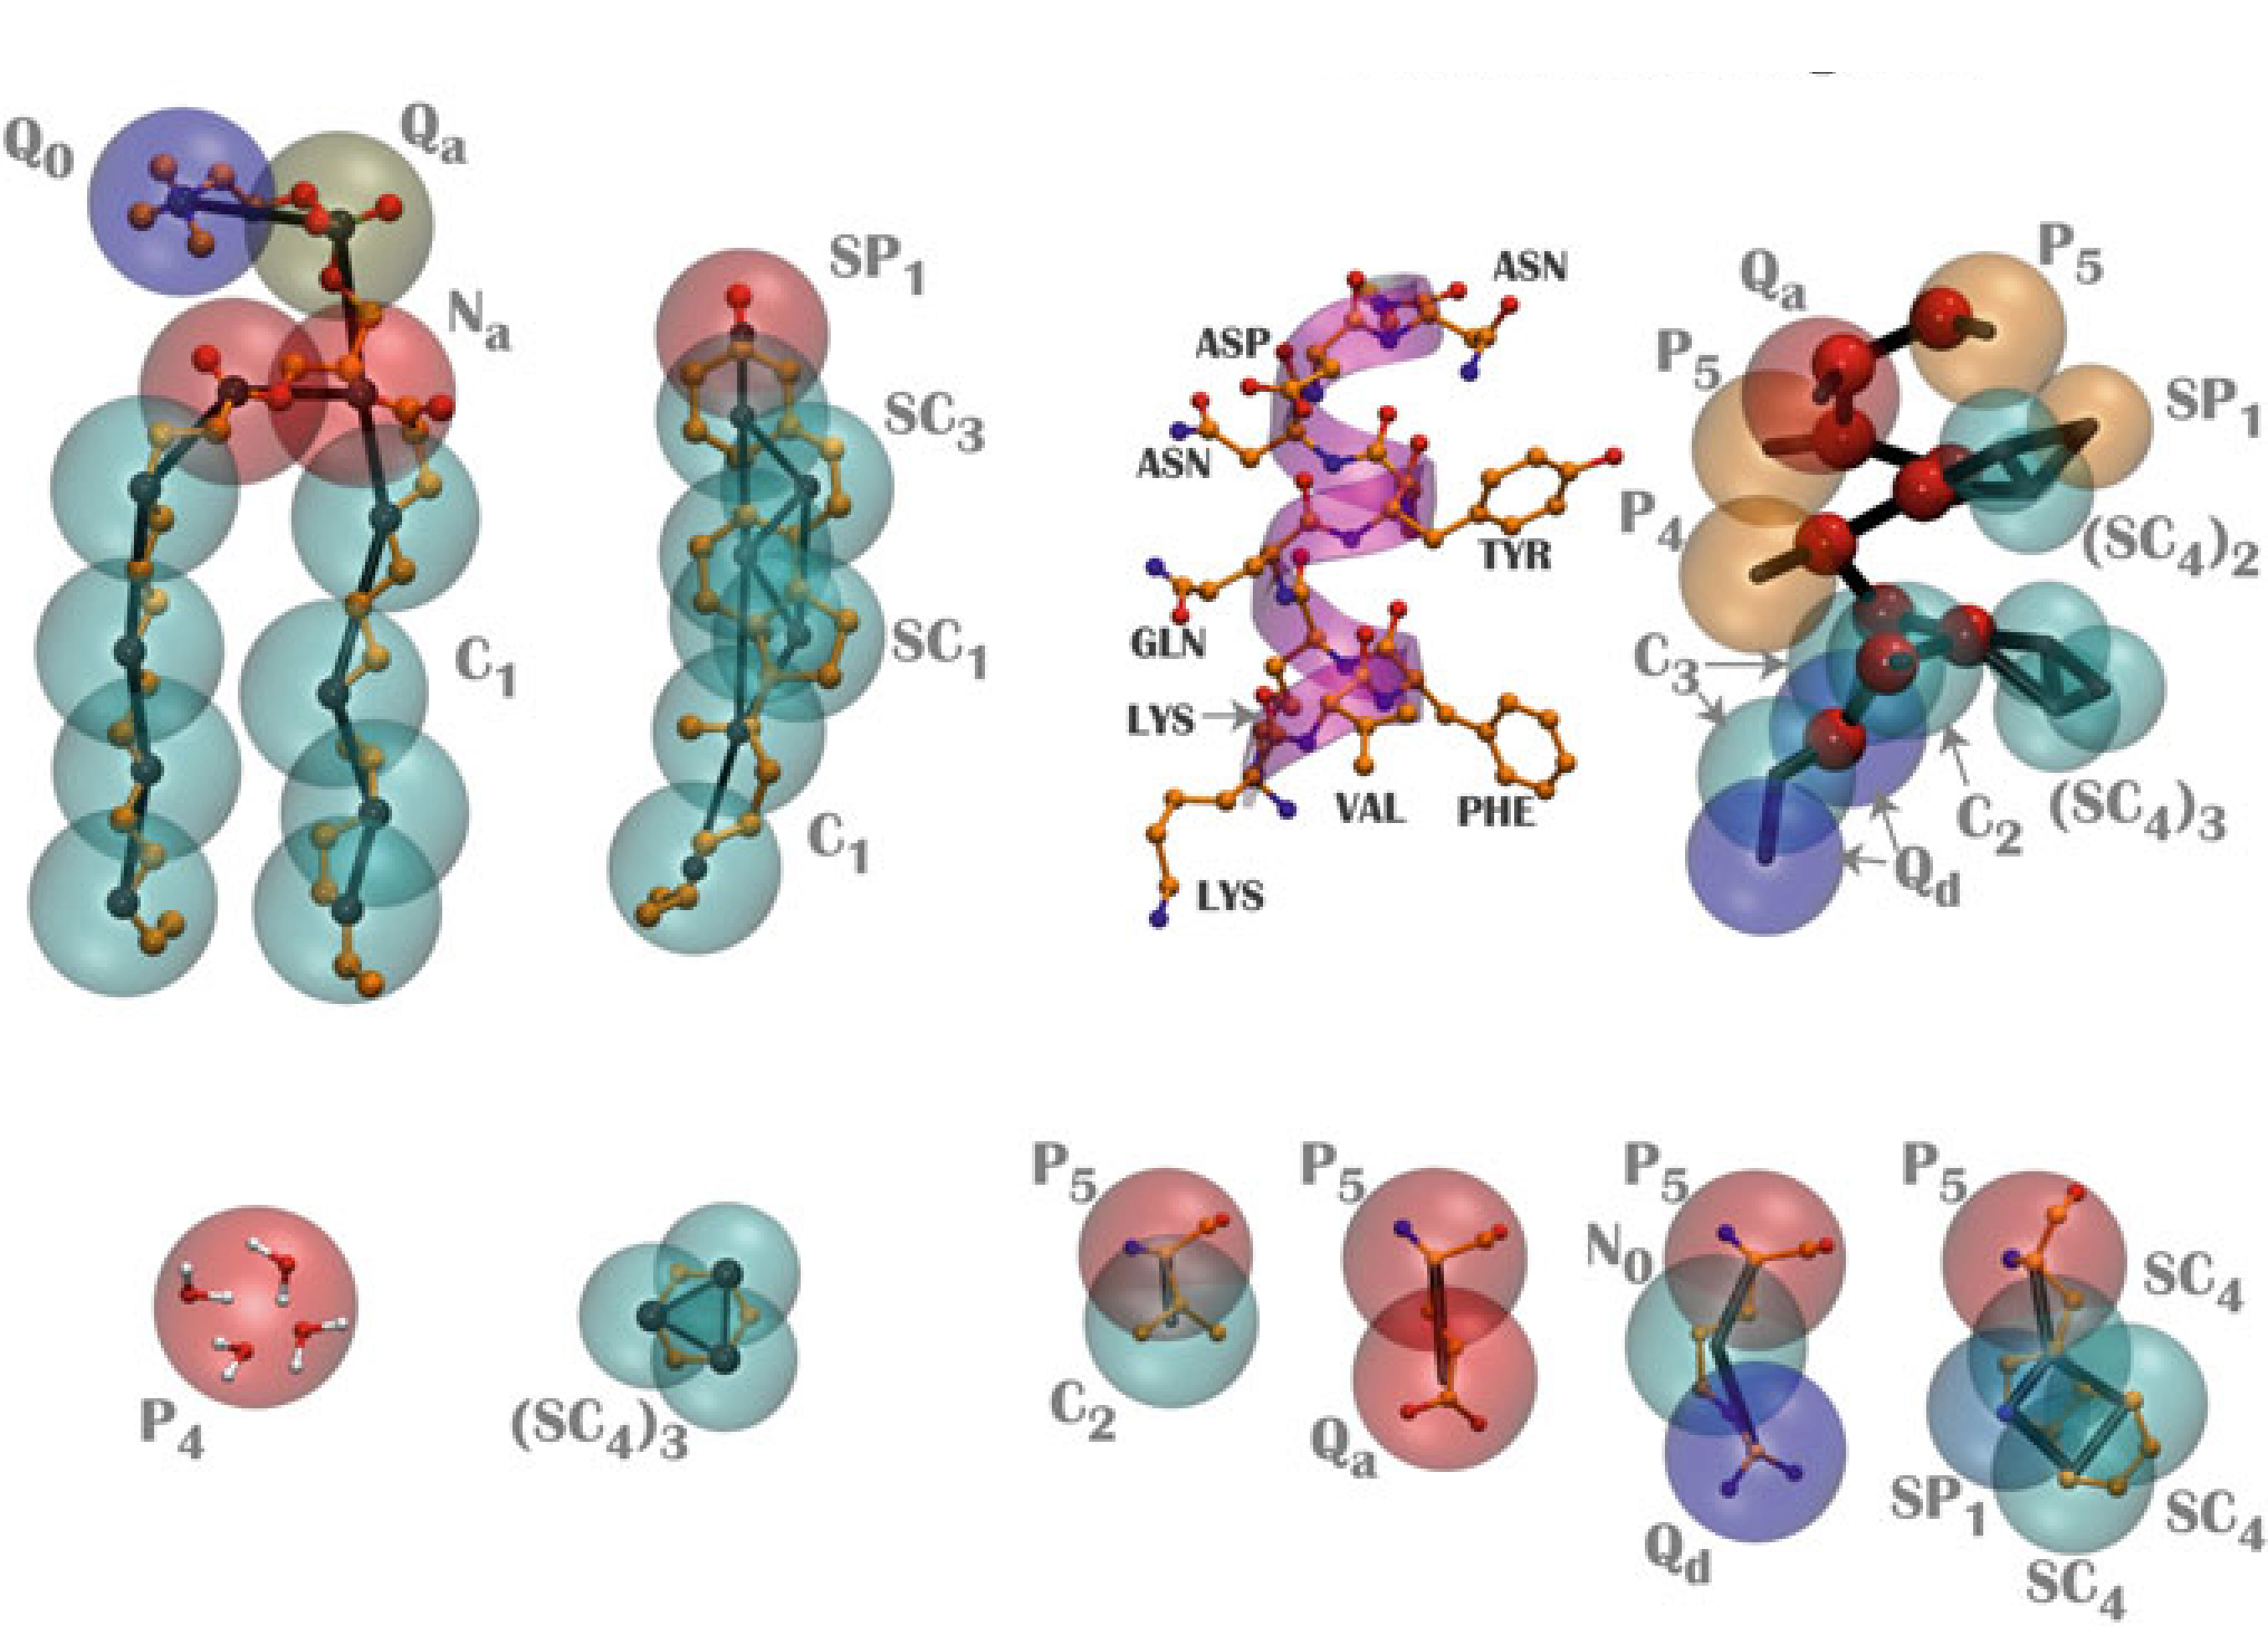
\includegraphics[width=.5\paperwidth]{martini-molecules}
    \end{center}
    
    \footnotesize{http://md.chem.rug.nl/cgmartini/index.php/about}

\end{frame}

\begin{frame}{Примеры систем из Martini}
    \begin{center}

      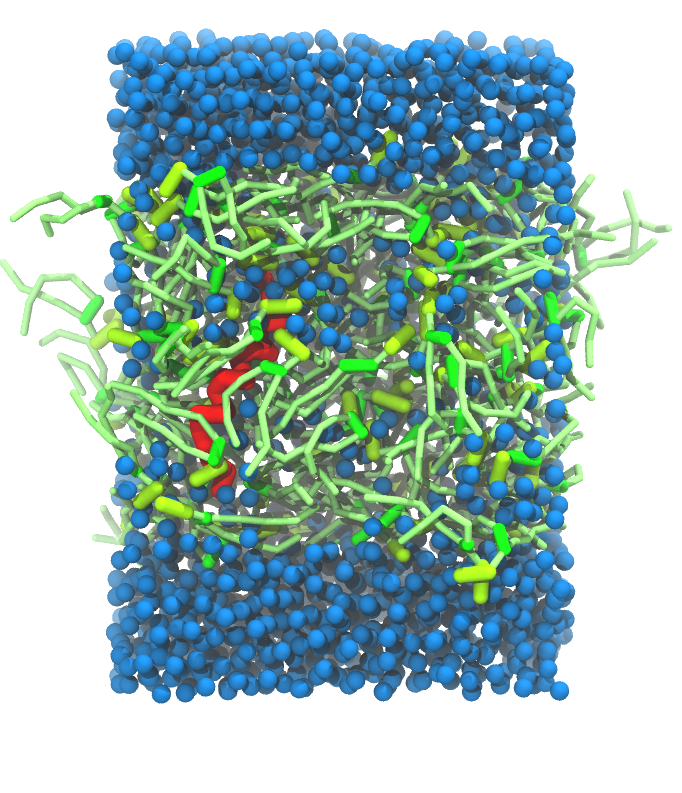
\includegraphics[width=.4\paperwidth]{kalp-cg_initial}
      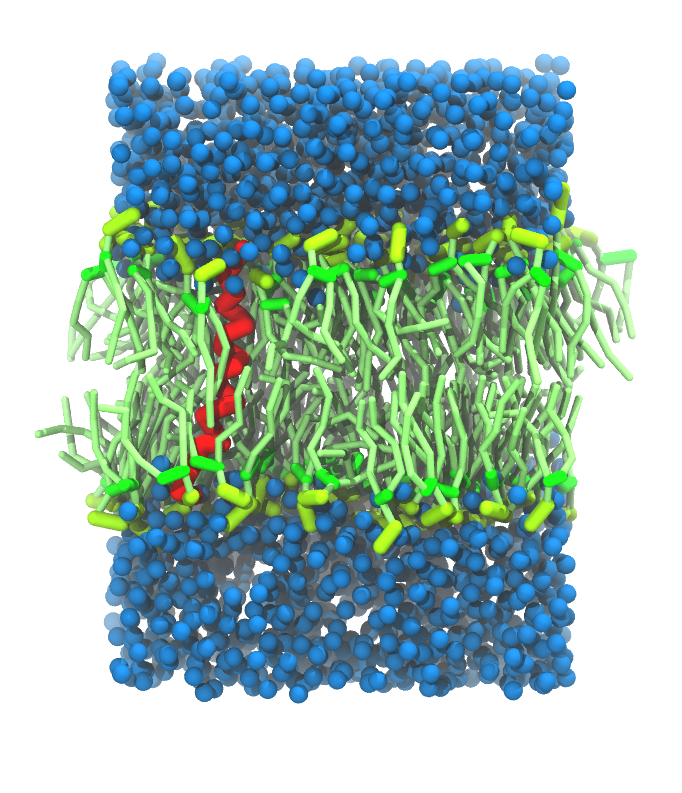
\includegraphics[width=.4\paperwidth]{kalp-cg_final.png}\\


    \end{center}

    \end{frame}   
\begin{frame}{Примеры систем из Martini}
    \begin{center}

      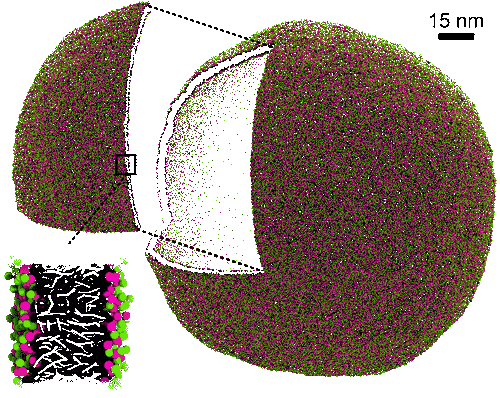
\includegraphics[width=.5\paperwidth]{martini-big}


    \end{center}
\end{frame}


\begin{frame}{Молекулярная механика твердого тела}
	$SiO_2$ - типичный объект подобных исследований. Часто бывает необходимо наблюдать дефекты в образовании кристаллической структуры.\\
	Ковалентную составляющую заменяют на модифицированные нековалентные потенциалы:
	\[ U= \sum_{i=1}^N \sum_{j=i+1}^N  \left (   4 \epsilon_{ij} \left [ \left ( \frac{\sigma_{ij}}{r_{ij}} \right )^{12} - \left ( \frac{\sigma_{ij}}{r_{ij}} \right )^6  \right ] + 
	\frac{q_i q_j}{ 4\pi \epsilon_0 r_{ij}} \right ) \]
	GlassFF:
	\[ U= \sum_{i=1}^N \sum_{j=i+1}^N \left( D_0 \left [ e^{{r(1-r_{ij}/r_0)}}  -2 e^{ \frac{r}{2}(1-r_{ij}/r_0)} \right ] + \frac{q_i q_j}{ 4\pi \epsilon_0 r_{ij}} \right ) 
	\]
\end{frame}



